\chapter{Survival Prognosis Replication: Methods}
\label{ch:study2_methods}

This chapter describes the methodology for Study~II, which replicates and extends the ALS survival prognosis framework of Papaiz et al.\ \cite{Papaiz2024}.
Study~I, which develops the original functional progression pipeline, is described in Chapter~\ref{ch:study1_methods}.
The two studies address different clinical targets and use different experimental designs; this chapter focuses exclusively on the survival prognosis task.

% ============================================================
\section{Rationale and Relationship to Study~I}
\label{sec:s2_rationale}
% ============================================================

Study~I develops an original leakage-free pipeline for predicting short-term ALSFRS-R functional progression in ALS.
Study~II addresses a different but complementary prognosis target: identifying patients who will die within 24 months of symptom onset, referred to throughout as Short Survivors.
Both studies share the same source database (\gls{PRO-ACT}), the same Optuna-based hyperparameter optimisation framework, and the same post-hoc SHAP interpretability approach, but they differ in their clinical target, feature set, class imbalance severity, and optimisation objective.

Study~II serves two purposes within this dissertation.
First, it extends the scope of ALS prognostic modelling from functional progression to survival prognosis, covering a second clinically relevant outcome.
Second, it evaluates reproducibility and methodological robustness by replicating and extending a published survival prediction pipeline under different validation and imbalance conditions.
Both purposes connect to the dissertation-wide themes: leakage-free validation, class imbalance, threshold-aware evaluation, explainability, and clinical interpretability.

% ============================================================
\section{Reference Study and Replication Objectives}
\label{sec:s2_reference}
% ============================================================

Papaiz et al.~\cite{Papaiz2024} proposed a systematic evaluation of six classical ML classifiers combined with BalancedBagging, using 23 hand-crafted clinical features derived from the PRO-ACT database.
That study (hereafter the \emph{reference study}) showed that the ensemble wrapper consistently improved balanced accuracy, with the MLP emerging as the best performer under repeated cross-validation.

The reference study left several methodological questions open: hyperparameters were tuned by grid search; gradient-boosted classifiers were not considered; and performance was assessed entirely within cross-validation without a separate held-out test set---a gap that, as this study's results show, has non-trivial consequences.

This study makes the following contributions:
\begin{enumerate}
  \item A partial replication of the reference study on the publicly available PRO-ACT extract, confirmed by Bonferroni-corrected statistical tests across all seven classifiers;
  \item An extension replacing grid search with Bayesian hyperparameter optimisation (Optuna~\cite{optuna2019}) and adding LightGBM~\cite{ke2017lightgbm} as a seventh classifier, evaluated across ten imbalance-handling strategies;
  \item A held-out test evaluation showing that the MLP's leading cross-validation AUC does not translate to adequate minority-class sensitivity at the default threshold, whereas LightGBM with Random Oversampling achieves the best overall balance;
  \item SHAP-based interpretability analysis~\cite{lundberg2017shap,lundberg2020treeshap} for both the replication and extension models, identifying diagnostic delay and ALSFRS-R decline slopes as the dominant prognostic variables.
\end{enumerate}

% ============================================================
\section{Dataset}
\label{sec:s2_dataset}
% ============================================================

\subsection{PRO-ACT Source and Cohort Construction}
\label{subsec:s2_proact}

The PRO-ACT database~\cite{PROACT} contains longitudinal clinical records from ALS patients enrolled across multiple controlled trials, covering ALSFRS-R assessments, vital signs, forced vital capacity (FVC), medication history, and demographic data.
The publicly available extract examined here comprises 2,147 patient records across 16 clinical tables prior to any filtering.
For the full description of PRO-ACT and its role in the thesis, see Section~\ref{subsec:methods_proact}; only the Study~II-specific differences are described here.

Following the feature engineering protocol of Papaiz et al.~\cite{Papaiz2024}, 23 categorical and ordinal features were extracted representing each patient's clinical status at or near the time of diagnosis.

\subsection{Target Definition}
\label{subsec:s2_target}

Throughout this study, patients who died within 24 months of symptom onset are termed \textbf{Short Survivors}; those who died after 24 months or were alive beyond that point are termed \textbf{Standard Survival} patients.
The binary target variable is defined accordingly: Short Survivor (death $\leq 24$ months from symptom onset) versus Standard Survival (death $> 24$ months, or alive beyond 24 months).
Patients alive at the time of their last observation but without 24 months of confirmed follow-up were treated as censored and excluded, consistent with the reference study.
Patients missing site-of-onset records were also excluded.

This target definition differs fundamentally from Study~I.
In Study~I, the target is the fold-wise binary classification of the ALSFRS-R slope---a continuous measure of short-term functional deterioration.
In Study~II, the target is confirmed death within a fixed 24-month window from symptom onset, a longer-horizon outcome with substantially more severe class imbalance.

\subsection{Cohort Size and Class Distribution}
\label{subsec:s2_cohort}

Table~\ref{tab:s2_dataset} compares the resulting dataset with the one reported in the reference study.
Our cohort comprises 1,502 patients, 23.6\% fewer than the original, primarily because the publicly available PRO-ACT extract contains a substantially higher proportion of missing FVC records (62.3\% after survival and site filtering) and sparser height data required for BMI derivation.
The imbalance ratio rises correspondingly (7.6 versus 6.9).

\begin{table}[ht!]
  \centering
  \caption[Dataset comparison with Papaiz et al.]{Dataset comparison between the reference study~\protect\cite{Papaiz2024} and Study~II.}
  \label{tab:s2_dataset}
  \begin{tabular}{lcc}
    \toprule
    \textbf{Metric} & \textbf{Papaiz et al.\ \cite{Papaiz2024}} & \textbf{Study~II} \\
    \midrule
    Total patients         & 1,967          & 1,502          \\
    Short Survivors (\%)   & 13.0\% (256)   & 11.6\% (174)   \\
    Standard Survival (\%) & 87.0\% (1,711) & 88.4\% (1,328) \\
    Imbalance ratio        & 6.9            & 7.6            \\
    Features               & 23             & 23             \\
    \bottomrule
  \end{tabular}
\end{table}

% ============================================================
\section{Feature Representation}
\label{sec:s2_features}
% ============================================================

\subsection{Preprocessing}
\label{subsec:s2_preprocessing}

Preprocessing mirrored the reference study's pipeline.
Binary features---sex, site of onset, riluzole use, and gastrostomy---were encoded as 0/1 indicators.
Age at onset was discretised into five ordinal groups ($\leq 39$, 40--49, 50--59, 60--69, $\geq 70$).
Diagnostic delay was categorised as short ($\leq 8$ months), average (9--18 months), or long ($\geq 19$ months), serving as a proxy for pre-diagnostic disease tempo.
FVC at diagnosis was classified as abnormal ($<$80\% predicted) or normal.
BMI was derived from body weight and height measurements closest to the diagnosis visit and encoded into four standard categories.

ALSFRS-R functional decline slopes for each of the ten subscores (Q1--Q10) were computed as $(4 - \text{score}) / \text{months from symptom onset}$ at the assessment visit closest in time to each patient's diagnosis date, following the formulation of the reference study~\cite{Papaiz2024}.
Where no pre-diagnosis assessment was available, the nearest available visit was used; this introduces a limited risk of post-diagnosis information being incorporated for a subset of patients, a limitation discussed in Section~\ref{sec:s2r_limitations}.
Slopes were binned as slow ($<$0.05), average (0.05--0.14), or rapid ($\geq$0.14 points per month).
Disease regions involved (bulbar, upper limb, lower limb, respiratory) were derived from ALSFRS-R subscores at the same visit.

\subsection{Feature Set}
\label{subsec:s2_featureset}

The final feature set comprises 23 features identical to those used by Papaiz et al.\ \cite{Papaiz2024}, all ordinal, binary, or categorical:

\begin{itemize}
  \item \textbf{Demographics (3):} Sex, Site of Onset (Bulbar / Limb / Other), Age at Onset (five ordinal groups).
  \item \textbf{Treatment and timing (2):} Riluzole use (binary), Diagnostic Delay (three ordinal categories).
  \item \textbf{Clinical severity at diagnosis (10):} FVC at diagnosis (binary), BMI (four categories), Gastrostomy (binary), five binary region-involvement flags (bulbar, upper limb, lower limb, respiratory, generalised), number of regions involved.
  \item \textbf{ALSFRS-R item slopes (8):} Functional decline slopes for items Q1 (speech), Q4 (handwriting), Q5 (cutting food), Q6 (dressing), Q8 (walking), Q9 (climbing stairs), Q10 (dyspnoea), and Q6 (turning in bed), each discretised into three ordinal categories.
\end{itemize}

These features differ from Study~I, which uses 35 baseline clinical features mostly continuous or mixed-type.
Study~II relies on pre-engineered ordinal and binary representations following Papaiz et al., enabling direct comparison with the reference study but constraining the feature space relative to Study~I.

% ============================================================
\section{Data Partitioning}
\label{sec:s2_split}
% ============================================================

The dataset was split 80/20 into training ($n = 1{,}201$; 139 Short Survivors, 1,062 Standard Survival) and test ($n = 301$; 35 Short Survivors, 266 Standard Survival) partitions using stratified random sampling (seed 42).
The test set was sealed until all model selection and hyperparameter optimisation had been completed.

% ============================================================
\section{Experimental Design}
\label{sec:s2_experiment}
% ============================================================

Figure~\ref{fig:s2_workflow} provides an overview of the complete experimental pipeline.

\begin{figure}[ht!]
  \centering
  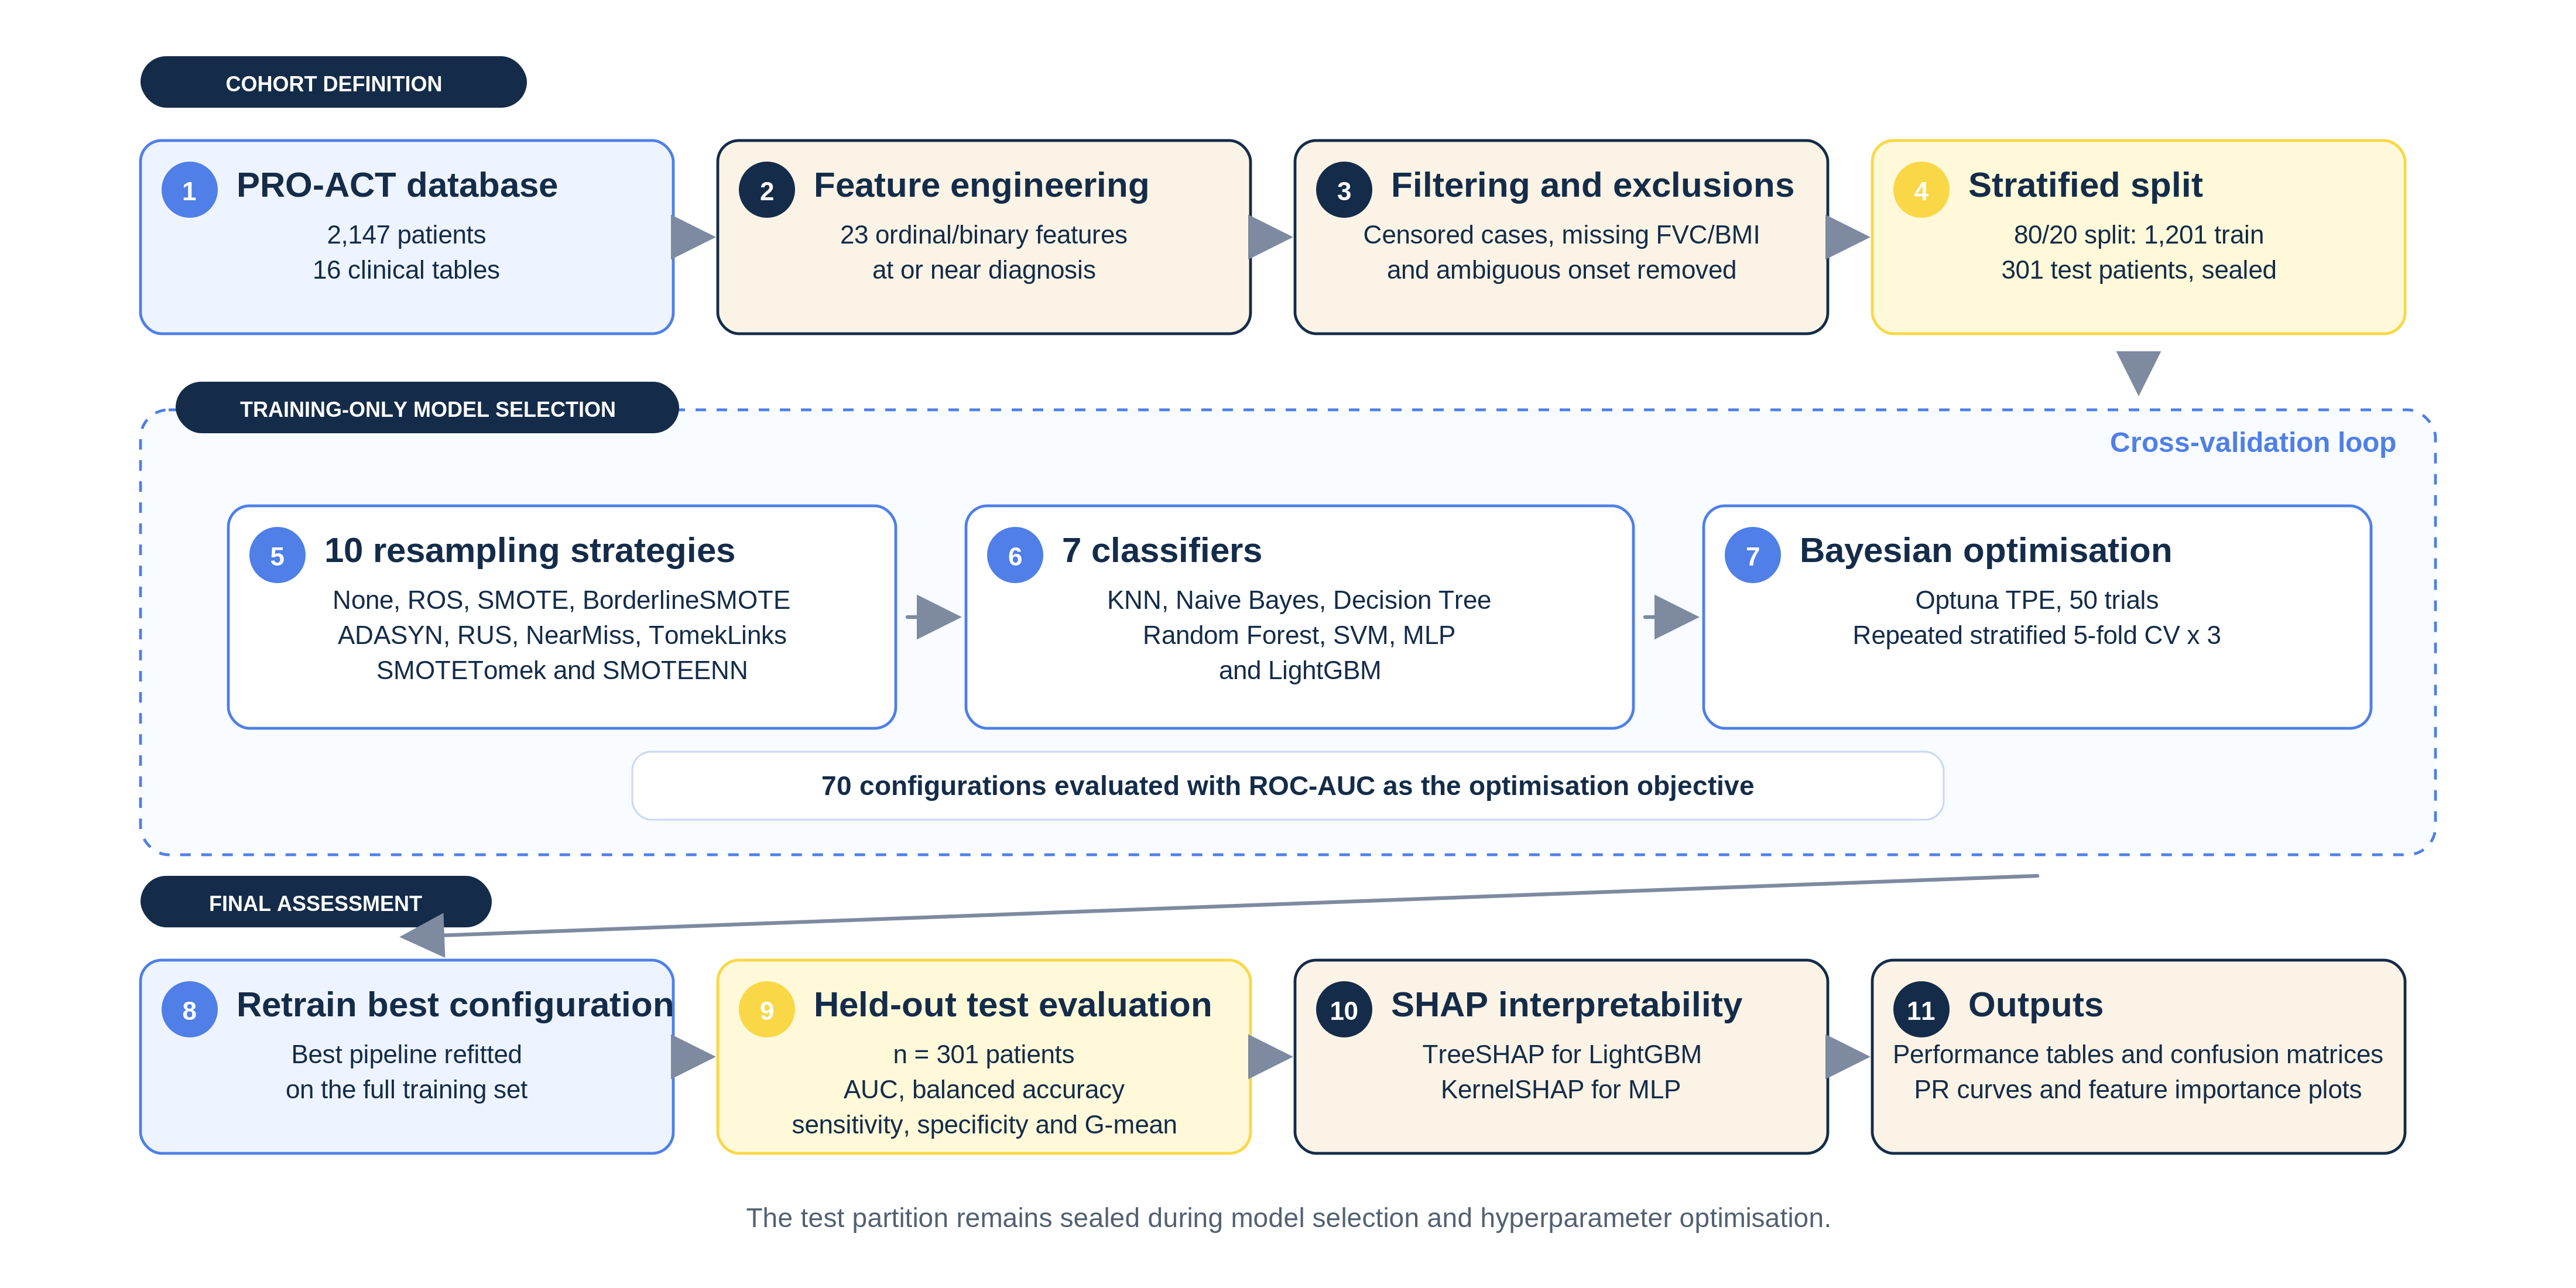
\includegraphics[width=\linewidth]{images/figures/experimental_pipeline.png}
  \caption[Study II experimental pipeline overview]{Overview of the Study~II experimental pipeline. The dashed border delimits the cross-validation loop, applied exclusively to the training partition. The test set remained sealed until all model selection and hyperparameter optimisation had been completed.}
  \label{fig:s2_workflow}
\end{figure}

\subsection{Classifiers and Imbalance Strategies}
\label{subsec:s2_classifiers}

Seven classifiers were evaluated: K-Nearest Neighbours (\gls{KNN}), Naïve Bayes, Decision Tree, Random Forest, Support Vector Machine (\gls{SVM}), Multi-Layer Perceptron (MLP), and LightGBM~\cite{ke2017lightgbm}.
The first six correspond directly to those used in the reference study; LightGBM is the primary extension.

Ten class-imbalance correction strategies were evaluated: no correction (None), Random Oversampling (ROS), SMOTE~\cite{chawla2002smote}, Borderline-SMOTE, ADASYN, Random Undersampling (RUS), NearMiss, TomekLinks, SMOTETomek, and SMOTEENN, yielding 70 classifier--strategy combinations in total.
All resampling operations were applied exclusively to the training fold of each cross-validation iteration, after the fold split and before classifier fitting; the validation fold and the held-out test set were never resampled.
Cross-validation estimates and final test performance therefore both reflect the natural class distribution (11.6\% Short Survivors), with no leakage from held-out samples into the resampled training distribution.

\subsection{Optimisation Protocol}
\label{subsec:s2_optuna}

Hyperparameter optimisation followed the same Optuna-based framework introduced in Study~I (Section~\ref{sec:methods_optuna}), employing the TPE sampler.
In Study~II, the protocol differed in three aspects: (i)~the objective metric was \gls{ROC-AUC} rather than \gls{PR-AUC}; (ii)~50 TPE trials were used per model--strategy combination rather than 60; and (iii)~optimisation was performed across 70 combinations, compared with 13 configurations in Study~I.

Optimising for the same criterion as the reference study (ROC-AUC) ensures that any divergence between cross-validation AUC and held-out minority-class performance can be attributed to properties of the criterion itself, not to differences in the model selection procedure.

\subsection{Cross-Validation Strategy}
\label{subsec:s2_cv}

Model selection was conducted using Repeated Stratified $K$-Fold cross-validation with $K = 5$ and 3 repeats (15 evaluations per configuration), applied exclusively to the training set.
Stratification ensures that class proportions are preserved in each fold.

This differs from Study~I, which uses a single 5-fold GroupKFold with subject-level separation.
Study~II uses repeated stratified CV because the replication framing follows the reference study's experimental design; each row corresponds to a distinct patient, so no explicit subject-grouping constraint applies beyond stratification.

% ============================================================
\section{BalancedBagging Replication Protocol}
\label{sec:s2_bagging}
% ============================================================

To directly replicate the reference study, all seven classifiers were additionally evaluated in two configurations using the same cross-validation protocol: (i)~a single-model baseline with no imbalance correction, and (ii)~wrapped inside a BalancedBagging ensemble~\cite{lemaitre2017} with ten estimators and random undersampling applied within each bootstrap iteration.

Per-fold balanced accuracy scores from the 15 cross-validation folds were compared between the single-model and BalancedBagging configurations for each classifier using the Wilcoxon signed-rank test~\cite{wilcoxon1945}.
Family-wise error rate inflation across the seven simultaneous comparisons was controlled by Bonferroni correction (corrected significance threshold $\alpha_c = 0.05 / 7 \approx 0.007$).

% ============================================================
\section{Explainability Protocol}
\label{sec:s2_xai}
% ============================================================

SHAP was applied as in Study~I (Section~\ref{subsec:methods_shap}) to provide post-hoc model explanations for survival prognosis.
TreeSHAP~\cite{lundberg2020treeshap} was used for the best LightGBM configuration, providing exact Shapley values at negligible computational cost.
KernelSHAP~\cite{lundberg2017shap} was used for the MLP model (100 background samples, 200 evaluation samples per instance), providing approximate Shapley values for a non-tree architecture.
SHAP values were computed on the held-out test set after final retraining on the full training partition.

% ============================================================
\section{Evaluation Metrics}
\label{sec:s2_metrics}
% ============================================================

Models were assessed using ROC-AUC, balanced accuracy, sensitivity (recall for the Short Survivor class), specificity, and geometric mean (G-Mean $= \sqrt{\text{Sensitivity} \times \text{Specificity}}$).
Missing a Short Survivor is the worst-case error in this clinical setting; sensitivity is therefore the primary metric throughout.

Given the small number of Short Survivors in the test set ($n = 35$), point estimates shift by 2.86 percentage points per patient.
Bootstrap 95\% percentile confidence intervals (2,000 resamples, \texttt{random\_state}$= 42$) were computed for all held-out metrics.
Bootstrap samples containing no Short Survivors were excluded from sensitivity and G-Mean calculations.

To investigate the effect of the decision boundary, three alternative thresholds were derived per classifier from out-of-fold (OOF) cross-validation predictions---never from the held-out test set---using (i)~Youden's J statistic~\cite{youden1950}, (ii)~the highest threshold achieving sensitivity $\geq 0.90$, and (iii)~the threshold maximising minority-class F1 score.
These thresholds were subsequently applied to the test set and evaluated alongside the default 0.50 boundary.

% ============================================================
\section{Methodological Differences from Study~I}
\label{sec:s2_differences}
% ============================================================

Table~\ref{tab:study_comparison} summarises the key methodological differences between the two studies.

\begin{table}[ht!]
\centering
\caption[Methodological comparison: Study I vs.\ Study II]{Methodological comparison between Study~I (functional progression) and Study~II (survival prognosis).}
\label{tab:study_comparison}
\small
\begin{tabular}{lll}
\toprule
\textbf{Dimension} & \textbf{Study~I} & \textbf{Study~II} \\
\midrule
Clinical target         & ALSFRS-R functional progression   & Survival $\leq 24$ months \\
Class distribution      & 30\% / 70\%                       & 11.6\% / 88.4\% \\
Imbalance ratio         & $\approx 2.3\!:\!1$              & $\approx 7.6\!:\!1$ \\
Features                & 35 (continuous + mixed)           & 23 (ordinal / binary) \\
Train / Test            & 1,113 / 279                       & 1,201 / 301 \\
Classifiers             & 7                                 & 7 (same families) \\
Imbalance handling      & Class-weight modes (2)            & Resampling strategies (10) \\
Total configurations    & 13                                & 70 \\
Tuning trials           & 60 per config                     & 50 per combo \\
Tuning metric           & \gls{PR-AUC}                     & \gls{ROC-AUC} \\
Validation strategy     & GroupKFold (5-fold)               & RepeatedStratKFold (5$\times$3) \\
Explainability          & SHAP + LIME + LR coefficients     & SHAP (TreeSHAP + KernelSHAP) \\
Contribution type       & Original model development        & Replication and extension \\
\bottomrule
\end{tabular}
\end{table}

